%=========PROBLEM 3============================================

\section*{Mode: Add wind}

This third mode will add wind to our system. 
\begin{equation*}
    \Sigma F = F_gravity + F_air + F_wind
\end{equation*}

The wind will have the same effect as the air resistance since they are both acting on a round object. For this reason we can use the same equation \ref{eq:drag} but now the velocity won't be the same as the golf ball. The wind's speed and direction will be determined by random uniform distribution. The speed will take values from 0 up to \SI{20}{\m\per\second} and the direction will be from 0 to $\pi$ where 0 is the direction from the golfer to the monkey, $\pi$ will be the direction from the monkey to the golfer and $\pi/2$ will be the vertical direction going downwards. To make these angles consistent with the angle of shooting, in my code I chose the range from 0 to $-\pi$. In addition, since I know that when the wind blows in the same direction as the movement of the bullet, the forces will add up and the opposite will happen when it goes against the movement. For these reasons, I let that my wind direction determine the 'minus' sign of the drag equation for the wind.

Figure \ref{fig:Wind} shows three plot in a similar way as the plot for air resistance mode. These plots show that there is no relevant difference between the system with added Air resistance only and the one with added air resistance and wind. This can be explained because the air resistance is proportional to square of velocity of the bullet i.e. $1100^2$ while the maximum speed of the wind is \SI{20}{\meter\per\second} which if squared is 400 not comparable to 1,210,000. 

\begin{figure}
    \centering
    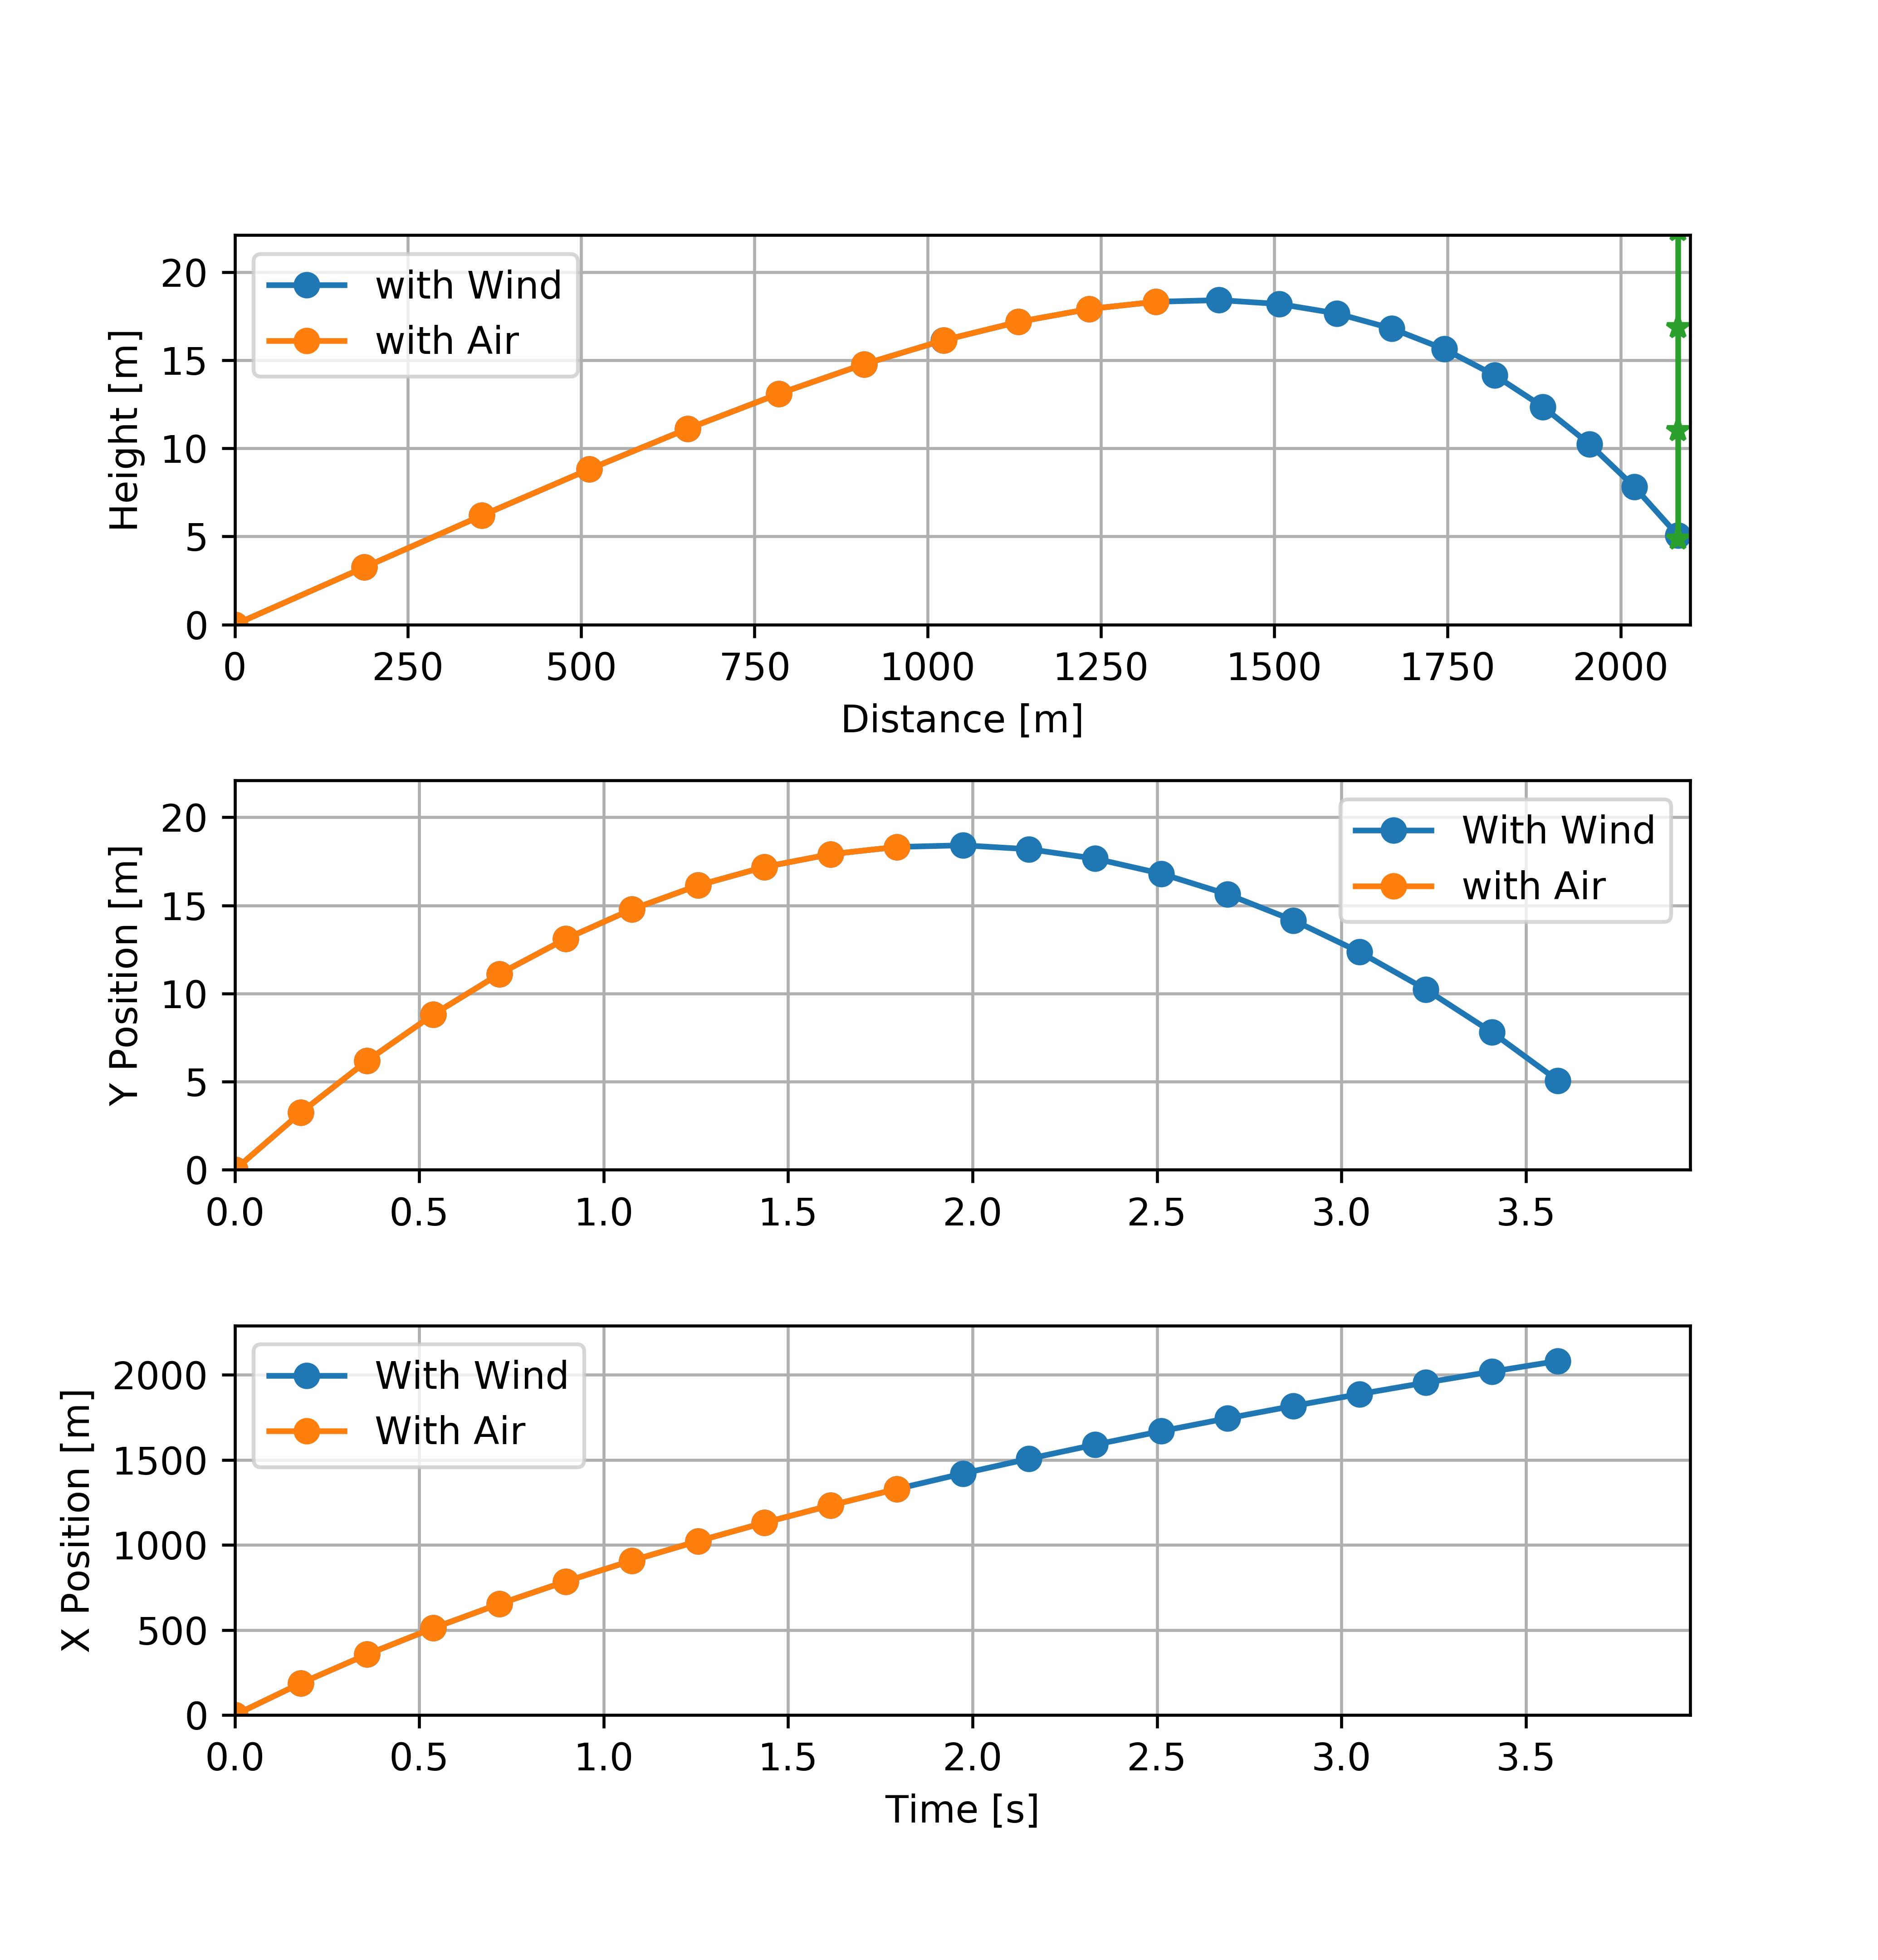
\includegraphics{figures/wa0-99x2082-44y67-97.png}
    \caption{Top: Shows the trajectory in terms of x and y position of the solution for the system with air resistance and with added air. Middle: Shows the y position in terms of time. Bottom: Show the x position in terms of time.}
    \label{fig:Wind}
\end{figure}

\section{Story Mode}
In addition to the previous modes, I added the story mode. The story mode allows my code to run as a game with a little story at the beginning. Then it asks you if air resistance and wind are present. After that, it allows you to aim to the monkey. After the calculation is done, it shows you the trajectory of the golf ball and the monkey. Finally, it determines if it was a HIT or a MISS. 

An example of the final plot is given in Figure \ref{fig:StoryMode}.

\begin{figure}
    \centering
    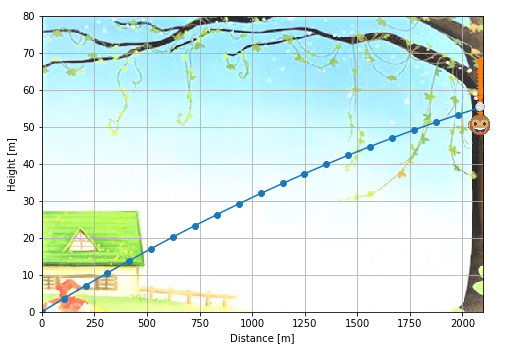
\includegraphics{figures/StoryMode.PNG}
    \caption{Example of the plot when using the Story Mode.}
    \label{fig:StoryMode}
\end{figure}

\section{Algorithm Complications}

The main complication that I had was to create a generic main while loop that will work for everything conditional to the modes. I start migrated some the sections of code into functions that can be called with different configurations. Then I realized that some function were using variables outside of their functions and start giving me errors. In the end, this process was taking too much time so I made individual whiles for each mode. 

The debugging process was made so much simpler when I start creating debug if's which will print values that I needed to assess the process. These if's are still kept in the code for future use by setting the debug variable into True. I know that there exist some error-catch commands which will do something similar. 

The interpolation was taking a lot of my time so I kept my code calculating values at steps of 0.0001 s. In my laptop, this loop takes about 2 seconds. This is another area of improvement.

I did try comparing my results with the ones given by odeint but realize that odeint was too optimized to make a true comparison. Also realized that the functions that I created were different structure than the ones required by odeint. This experiment showed me the advantages of using function already tested and optimized. 
